\section*{Metode}
\label{Metode}
%
Indenfor \textit{Multidimensional Scaling}, (MDS), findes der tre standard metoder, der kan anvendes: \textit{Classical MDS}, \textit{Non-classical MDS} og \textit{Non-metric MDS}. Hvilken af de tre metoder, der anvendes afhænger af den indsamlede datatype. Er data på interval niveau anvendes \textit{Classical MDS}, som ydermere anvender lineær algebra og kræve et fuldt datasæt, hvor samtlige kombinationer er præsenteret. Er dette ikke tilfældet kan \textit{Non-classical MDS} anvendes, da metoden ikke kræver lineær algebra men derimod tillader iterative algoritmer. Derudover er det ikke en forudsætning at det er et fuldt datasæt. Er data derimod på ordinal niveau anvendes \textit{Non-metric MDS}, ved denne metode analyseres data på samme måde som ved \textit{Non-classical MDS}, hvorfor data først skal transformeres fra ordinal til interval data, \parencite[s. 9]{Wickelmaier2003}. 

Da data indsamlet i dette eksperiment er ordinal data vælges det, at analysere data med metoden \textit{Non-metric MDS}.\blankline
%
Ved MDS skal antallet af dimensioner bestemmes. For at vurdere hvor godt det valgte antal dimensioner passer på data, anvendes begrebet \textit{Stress}, som er et udtryk for hvor godt de reelle forskelle er repræsenteret.

Antallet af dimensioner vælges ud fra et kompromis mellem hvor let det skal være at fortolke data og hvor lidt \textit{stress} der skal være. Desto flere dimensioner der vælges, desto svære bliver det at fortolke data, med samtidig vil der opnåes mindre \textit{stress}. \autoref{fig:TolkningStress} illustrer sammenhængen mellem \textit{stress}-værdien og hvor godt fit'et er. 
%
\begin{figure}[H]
\centering
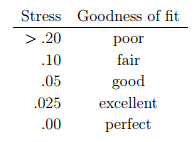
\includegraphics[width = 0.25\textwidth]{Figure/TolkningStress.PNG} 
\caption{Sammenhæng mellem \textit{stress} og hvor godt fit'et er, \parencite[p.13]{Wickelmaier2003}.}
\label{fig:TolkningStress}
\end{figure}	
%

